%; whizzy paragraph -pdf xpdf -latex ./whizzypdfptex.sh
%; whizzy-paragraph "^\\\\begin{frame}"
% latex beamer presentation.
% platex, latex-beamer でコンパイルすることを想定。 

%     Tokyo Debian Meeting resources
%     Copyright (C) 2011 Junichi Uekawa
%     Copyright (C) 2011 Nobuhiro Iwamatsu

%     This program is free software; you can redistribute it and/or modify
%     it under the terms of the GNU General Public License as published by
%     the Free Software Foundation; either version 2 of the License, or
%     (at your option) any later version.

%     This program is distributed in the hope that it will be useful,
%     but WITHOUT ANY WARRANTY; without even the implied warreanty of
%     MERCHANTABILITY or FITNESS FOR A PARTICULAR PURPOSE.  See the
%     GNU General Public License for more details.

%     You should have received a copy of the GNU General Public License
%     along with this program; if not, write to the Free Software
%     Foundation, Inc., 51 Franklin St, Fifth Floor, Boston, MA  02110-1301 USA

\documentclass[cjk,dvipdfmx,12pt]{beamer}
\usetheme{Tokyo}
\usepackage{monthlypresentation}

%  preview (shell-command (concat "evince " (replace-regexp-in-string "tex$" "pdf"(buffer-file-name)) "&")) 
%  presentation (shell-command (concat "xpdf -fullscreen " (replace-regexp-in-string "tex$" "pdf"(buffer-file-name)) "&"))
%  presentation (shell-command (concat "evince " (replace-regexp-in-string "tex$" "pdf"(buffer-file-name)) "&"))

%http://www.naney.org/diki/dk/hyperref.html
%日本語EUC系環境の時
\AtBeginDvi{\special{pdf:tounicode EUC-UCS2}}
%シフトJIS系環境の時
%\AtBeginDvi{\special{pdf:tounicode 90ms-RKSJ-UCS2}}

\title{東京エリアDebian勉強会}
\subtitle{第83回 2011年12月度}
\author{野島 貴英 nozzy@debian.or.jp\\IRC nick: nojima\\twitter: nozzy123nozzy}
\date{2011年12月17日}
\logo{
\includegraphics[width=8cm]{image200607/openlogo-light.eps}}

\begin{document}

\frame{\titlepage{}}


\begin{frame}{設営準備にご協力ください。}
会場設営などよろしくおねがいします。
\end{frame}


\section{Agenda}
\begin{frame}{Agenda}
\begin{minipage}[t]{0.45\hsize}
  \begin{itemize}
  \item 注意事項
	\begin{itemize}
	 \item 飲酒禁止
	 \item 宗教禁止
	 \item 営利活動禁止
	\end{itemize}
   \item 最近あったDebian関連のイベント報告
	\begin{itemize}
        \item 第81回 東京エリアDebian勉強会(筑波)
        \item 第82回 東京エリアDebian勉強会(OSC)
	\end{itemize}
 \end{itemize}
\end{minipage} 
\begin{minipage}[t]{0.45\hsize}
 \begin{itemize}
   \item Debian Trivia Quiz
   \item 事前課題紹介
   \item 2011年の振り返り
   \item quiltでportingしてみた
   \item 月刊Debhelper 第2回
  \end{itemize}
\end{minipage}
\end{frame}

\section{イベント報告}
\emtext{イベント報告}
\emtext{東京エリアDebian勉強会(筑波)}

\begin{frame}{東京エリアDebian勉強会 in 筑波}
\begin{itemize}
\item 開催場所は 筑波大学
\item 10/22 (土)13時に現地集合
\item 学生さんも参加されました。
\item Debianユーザ寄りの発表が多め?でした。
\end{itemize}
\end{frame}

\emtext{東京エリアDebian勉強会(OSC)}

\begin{frame}{東京エリアDebian勉強会 in OSC 2011 Tokyo/Fall}
\begin{itemize}
\item 開催場所は 明星大学
\item 11/19(土) 11:00-11:45で最近のDebianについてのセッションが行われました。
\item ブースを開きました(2日間) LiveCDも配りました。
\end{itemize}
\end{frame}

\section{DWN quiz}
\emtext{DWN quiz}
\begin{frame}{Debian 常識クイズ}

Debian の常識、もちろん知ってますよね?
知らないなんて恥ずかしくて、知らないとは言えないあんなことやこんなこと、
みんなで確認してみましょう。

今回の出題範囲は\url{debian-devel-announce@lists.debian.org},
\url{debian-devel@lists.debian.org} に投稿された
内容とDebian Project Newsなどからです。

\end{frame}

\subsection{問題}
%; whizzy-master ../debianmeetingresume201101.tex
% $B0J>e$N@_Dj$r$7$F$$$k$?$a!"$3$N%U%!%$%k$G(B M-x whizzytex $B$9$k$H!"(Bwhizzytex$B$,MxMQ$G$-$^$9!#(B
%
% $B$A$J$_$K!"%/%$%:$OJL%V%i%s%A$G:n@.$7!"$N$A$K%^!<%8$7$^$9!#5U$K%^!<%8$7(B
% $B$J$$$h$&$K$7$^$7$g$&!#(B
% (shell-command "git checkout quiz-prepare")

\santaku
{11$B7n=*$o$j:"$K%k!<%H%U%!%$%k%7%9%F%`$N9=B$$K$D$$$F5DO@$r8F$s$G$^$9!#FbMF$O!)(B}
{/user$B$r:n$k(B}
{/bin,/sbin,/lib$B$N<BBN$r(B/usr$B0J2<$K0\F0$7$F!"Be$o$j$K%7%s%\%j%C%/%j%s%/$K$9$k(B}
{/etc$B$N<BBN$r(B/usr$B0J2<$K0\F0$7$F!"Be$o$j$K%7%s%\%j%C%/%j%s%/$K$9$k(B}
{B}
{$BB><gMW%G%#%9%H%j%S%e!<%7%g%s$,:NMQ8!F$Cf(B...}

\santaku
{sun-java6$B$,(BDebian$B%Q%C%1!<%8$H$7$FG[I[$G$-$J$/$J$j$^$7$?!#Be$o$j$K(BDebian$B$G?d>)$5$l$k(BJava$B$O(B?}
{openjdk}
{gcj-jdk}
{coco-java}
{A}
{$B;DG0$@!d!{(Bracle}

\santaku
{11/19$B$KD9$i$/3hF0$rDd;_$7$F$$$?%Q%C%1!<%8%A!<%`$,I|3h@k8@$r$7$^$7$?!#$I$l$G$7$g$&!)(B}
{CORBA packaging team}
{Ham-radio packaging team}
{SDL packaging team}
{C}
{$B$3$l$+$i$b4hD%$C$FM_$7$$$G$9$M(B}

\santaku
{10/28$B!A(B30$B$G(BMiniDebconf2011$B$,3+$+$l$^$7$?!#$I$3$N9q$G$7$g$&!)(B}
{$B%K%+%i%0%"(B}
{$B%$%s%I(B}
{$B%U%i%s%9(B}
{B}
{$BMhG/$OF|K\$,$$$$$J$!(B}

\santaku
{Wheezy$B%U%j!<%:$N0Y$N(BBSP$B$,3F9q$G3+$+$l$^$7$?!#%I%$%D$H$I$3!)(B}
{$B%U%i%s%9(B}
{$B%K%+%i%0%"(B}
{$B%]!<%i%s%I(B}
{C}
{Wheezy$B$N%U%j!<%:$O(B2012/6$B$J$N$G!"3+H/:n6H$O$*Aa$a$K(B}



\section{事前課題}
\emtext{事前課題}
{\footnotesize
 \begin{prework}{Kazuo Ishii}
emacs $B>o$K%+%9%?%^%$%:$rB3$1$F$$$^$9!#$3$l$r$I$l$@$1;H$$$3$J$9$+$,!"2]Bj$G$9!#(B
\end{prework}
\begin{prework}{Aru}
\begin{itemize}
\item postfix$B$N%=!<%9%3!<%I$r$$$8$C$F%Q%C%1!<%82=$5$;$F%$%s%9%H!<%k$7$J$*$7$^$7$?!#(B
\item $B!{(BCN$B$N2s@~>e$G(BSMTP$B%5!<%P$r9=C[$9$k:]$O(BOP25B$B$N4X78>e(BOCN$B$N(BSMTP$B%5!<%P$rDL$5$J$1$l$P$J$i$J$$$N$G$9$,!"$=$N(BSMTP$B%5!<%P$,FC<l$J;EMM$N$h$&$G(Bpostfix$B$N@_Dj$rJQ$($k$@$1$G$O%5!<%P$KCF$+$l$F$7$^$$$^$9!#$=$3$G!"!{(BCN$B$N%5!<%P8~$1$K%=!<%9%3!<%I$r$$$8$j$^$7$?!#(B
\end{itemize}
\end{prework}

\begin{prework}{koedoyoshida}
\begin{itemize}
\item Unbound:\\
$B;E;v$GI>2AMQ(BDNS$B$r7z$F$k$N$K;H$C$?$j!"(Bdnstudy$BEy$GH/I=$N4m81$J(BLT$B%M%?$H$7$F;HMQ!#(BBIND$B$KHf$Y$FNI$/$G$-$F$k$N$GFC$K2]BjEy$O$J$7(B
\item zabbix:\\
$B4pK\(Bstable$B$r;H$C$F$$$k$3$H!"$+$DH/E8ES>e$N%=%U%H$G$"$k$3$H$+$iK-IY$J$O$^$j%]%$%s%H$,M-$C$?!#$,4pK\E*$K$0$0$C$F2r7h$7$?$j!"I=<(>e$NLdBj$J$N$GL5;k$7$?$j$7$F$^$9!#(B\\
\end{itemize}
\end{prework}

\begin{prework}{yamamoto}
\begin{itemize}
\item $B:#G/%Q%C%1!<%82=$7$?(BDebian$B%Q%C%1!<%8(B: $BL5$7(B \\
$B$&!<$`!"<+J,@lMQ$N%Q%C%A$r$"$F$?%+!<%M%k%Q%C%1!<%8$0$i$$$C$9$M!#(B
$B9W8%$O$G$-$F$J$$$J!#(B

\item $B:#G/;H$$9~$s$@(BDebian$B%Q%C%1!<%8(B: devscripts pbuilder \\
devscripts $B$G%]%A%]%A$H(B sbuild $BMQ$K%Q%C%1!<%8$r:n$j!"(Bpbuilder $B$G:F%S%k%I$7$F$^$7$?!#(B
$B:#G/$O(B FTBFS $B$rD>$7$F$b$i$&(B BTS $B$r$?$^$K$9$k$N$H!"<+J,@lMQ%j%]%8%H%j$r:G?7$K(B 
$BJ]$D$@$1$G!"$$$C$Q$$$$$C$Q$$$G$7$?!#(B

\item $BMhG/;H$$9~$`M=Dj$N(BDebian$B%Q%C%1!<%8(B: sbuild buildd \\
$B$5$F!"CF$,$G$-$?$7!"FM7b$8$c!<!#(B
\end{itemize}
\end{prework}
\begin{prework}{henrich}
$B:#G/$O$"$^$j%Q%C%1!<%8$r$$$8$/$C$F$J$$$G$9!D%Q%C%1!<%82=$7$?$b$N$H(B 
$B$$$($P(BIRC$B%/%i%$%"%s%H$N(Bloqui$B$H$+$0$i$$$G$7$g$&$+!#$=$l$b(Bupstream$B$NJ}$,!"$[$H(B 
$B$s$I?w7A:n$C$F$$$?$@$$$F$$$?$N$G:Y$+$$=j$rD>$7$?$@$1$G$7$?!#(B

DEP5$B$X$NBP1~$dB>$N(BDEP$B$X$NBP1~$J$I$,:#8e%Q%C%1!<%8%/%*%j%F%#$r5s$2$k>e$G2]Bj(B 
$B$G$7$g$&$+!J<g$KLLE]$/$5$$0UL#$G!K(B
\end{prework}
\begin{prework}{$B$^$($@$3$&$X$$(B}
 12/8$B;~E@$N>u67(B
\begin{itemize}
\item $B%Q%C%1!<%8%s%0:Q$_(B
\begin{itemize}
\item python-funcparserlib : $B%F%9%H$G%3%1$kLdBj(B
\item python-webcolors
\end{itemize}
\item $B%Q%C%1!<%8%s%0ESCf(B
\begin{itemize}
\item python-ordereddict$B!'(BPython2.6$B$N$_(B
\item python-blockdiag : Python 2.6$B$O(Bpython-ordereddict$B$r!"(B2.7$B$OAH$_9~$_$N(B 
ordereddict$B$r;H$&$h$&$K%Q%C%1!<%8%s%0$9$k$K$O(Bdebian/control$B$I$&=q$1$P$$$$$s(B 
$B$@!)(B
\item python-{sec,act,nw}diag$B$*$h$S(B 
python-sphinxcontrib.{block,seq,act,nw}diag : python-blockdiag$BBT$A(B
\item python-tomahawk : nodetests$B$G%3%1$kLdBj(B
\end{itemize}
\end{itemize}
\end{prework}


}
\section{今月の発表}
\subsection{2011年の振り返り}
\emtext{2011年の振り返り}

\begin{frame}{参加者数、事前・事後課題 年移動平均推移}
 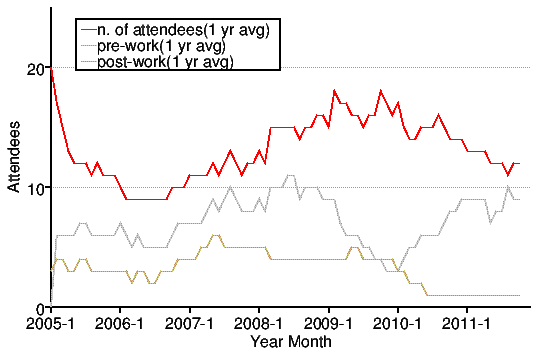
\includegraphics[width=0.7\hsize]{image201112/memberanalysis/attend.png}
\begin{itemize}
\item 参加者数は下降傾向
\item 事前課題は横ばい傾向\\
  事前課題をちゃんと出す=常連参加者に収斂?
\item 事後課題(ブログ)の率はさらに低下
\end{itemize}
\end{frame}

\begin{frame}{2011年参加者数実績}

{\tiny
  \begin{tabular}{|l|c|c|l|}
 \hline
 & 参加人数 & 場所 & 内容\\
 \hline
1月 & 12 & 荻窪 & Kinect,アンケートシステム,CACertサイン会 \\
2月 & 13 & 北新宿生涯学習館 & HDFS,Debian Game Team \\
3月 & ? & OSC & CACert ATE Tokyo \\
4月 & 12 & IIJ & backports,initramfs,月刊PPC64 \\
5月 & 15 & 戸山生涯学習館 & Apache2モジュール,Debian on ニフクラ,Debian/m68k \\
6月 & 17 & オリンピックセンター & ドキュメント処理系, 2011再計画 \\
7月 & 3 & ボスニア & DebConf11 \\
8月 & 12 & 荻窪 & パッケージング関連, Debconf11報告 \\
9月 & 9 & 山喜旅館 & Debian温泉2011 \\
10月 & 22 & 筑波大学 & Haskell,LaTeX,レポート自動生成,月刊Debhelper開始 \\
11月 & ? & OSC & CACert \\
12月 & 9 & SQUARE ENIX & quiltでporting,月刊Debhelper \\
 \hline
  \end{tabular}
}

\begin{itemize}
{\scriptsize
\item 昨年同様、人数的には大きく増減はない
\item OSCにならび、大学での開催時は参加者数および初参加者が増加
\item 毎月数名は初参加者いる。うち一部は2回目以降も参加\\
  ちゃんと事前課題を提出する人が常連になる傾向?
\item あんさんぶる荻窪以外の公民館などの利用が増加
\item 三回目のDebian温泉。伊東の山喜温泉で開催
\item Debian Hack Cafeも月1ペースで再開
}
\end{itemize}
事前課題の提出率は維持しつつ、参加者数は増やしていく為の対策は必要
\end{frame}

\begin{frame}{2011年の成果}

{\tiny
\begin{tabular}{|c|c|c|}
\hline
& 2010 & 2011 \\
\hline
DDになった人 & やまねひでき & \\
NM & kiwamu, 上野だいき & \\
DM & kurashiki, kiwamu, uwabami... &\\
Debian JP 加入 &  1人 & 4人(東京2人) \\
\hline
\end{tabular}
} 
\end{frame}

\begin{frame}{タイムライン 書き直そう!}

{\tiny
\begin{tabular}[t]{|p{8.5em}|p{12em}|p{8em}|p{6em}|p{8em}|}
\hline
2008 &2009 & 2010 & 2011 & 2012 \\
\hline
%2008

python3.0
ruby1.9

wine1.0, wine64

RoR2.0 で普及に

4コア64bitCPU, Core2Quad普及

ニコニコ動画1000万ユーザ
初音ミクブーム

地デジ関連のPC製品普及

勉強会普及

公衆無線LAN

携帯電話の売上落ちる
iPhone, Android 登場

emobile 100円PC抱きあわせ
Zaurus販売終了

サーバの仮想化 ESXi, シンクライアント

MacBook Air 発売

世界経済の崩壊(IT投資緊縮財政、失職者増加)

FreeBSD7

Debian次世代育成計画始動
Debian Maintainer 制度始動

セキュリティー関連(OpenSSL事件、DNS事件)

クラウド関連が流行?

&
%2009
政権交代, スパコン事業仕分け, 円高

Windows7, Snow Leopard

Netwalker, Eye-Fi, Kindle2, DS LL, PSP-GO, POKEN

MacBookのIEEE1394終了, Cell終了

ラブプラス, OSSを使ったエロゲー登場(OpenCV), AR, セカイカメラ, マジコン販売取締り, デジタルサイネージ

JLSでLinus来て大騒ぎ

DD, 2世誕生, Debian 結婚ブーム, Lenny リリース

Google Voice, Wave, Chrome, Chrome OS, Go, 日本語入力, 徒歩ナビ
Twitter, *なうブーム

tile window manager, CouchDB

デスクトップ4コア8GB, ノートPC 2コア4GB, メモリDDR3に移行中, メモリ高騰

Linux が標準インストールのPC(Dell)

SSD の値段と容量がこなれる(まあまあ)
HDDがなくなる?高くなる?(ならず)

SSD特化したFSが出てきた

IPv6 使えるようになってる(来年)

DL禁止法? torrent に逆風?

&
%2010

Toystory 3

デスクトップPC:QuadCore普通

DDR3 安い 8GB 8000円

ノートパソコン:
NetBookかとおもいきやタブレットPCが普及

iPhone4, iPad

Willcom再生(Softbankに)

Sun終了

% はやぶさ帰還、あかつき失敗

% NTT vs Softbank 光の道

% 今年も首相交代

自炊ブーム, 電子書籍, kindle とか

kFreeBSD リリースされそう
zfs がデフォルトで選べる

BtrFSこなかった, ext4 きた

IS01祭り, Android祭り

ARM 全盛

クラウド流行

KVS大流行

% Willcom -> Softbank
% SSD
% SIm lock free not yet
% Android だらけ
% Netbook涙目、iPad タブレット盛り上がり
% Cloud!
% iPhone4
% 民主終了、自民は???
% ext4がきた
% kFreeBSDが本当にリリースアーキテクチャになりそう
% Toystory 3 はきた。
% 消費税まだあがっていない
% USB 3.0 なにそれ
% ARM 全盛、Atomあまり普及せず。
% ruby 2.0 なにそれ


&
%2011

デスクトップ終了?
高速化しない

ノートパソコン:
ChromeOS?
Android?

webOS終了のお知らせ?(終了\&復活?)

Adobe Flash復活のお知らせ(キタ), Silverlight終了のお知らせ(台湾を除く)(続いてる?)

Squeezeリリース(おめでとう)

IPv4割り当ての終了のお知らせ(キタ)

地上波デジタル移行延長(無い?)

Btrfsまだ頑張る(Fedora乙)

Java終了(Sub Java終了)

Open OfficeがOracle Officeに(ナイ)

&
%2012

デスクトップ:終了している。

サーバ:
光インターコネクト?VPS以外はない?

ノートパソコン:Intelじゃないもの(MIPS/ARM)が主流に。

携帯電話:
ガラパゴスの終焉。
LTEが主流になっていない。
Softbankの二年契約が終了、SIM Freeがあたりまえに?

日立と東芝ハードディスク事業を売却統合?

液晶が絶滅。

OracleがBtrfsを終了させる

MySQLがOraSQLに

% Mixi炎上、Facebookが救済、か?

MacBookが新しい基盤に。

\\

\hline
\end{tabular}

}
\end{frame}

\begin{frame}{2012,2013年を予想してみよう}

{\tiny
\begin{tabular}[t]{|p{20em}|p{20em}|}
\hline
2012 & 2013 \\
\hline

%2012

ARMサーバでたけど微妙

デスクトップがノートの1/10

ノートがタブレットに抜かれる

ノートのCPUがARM,MIPS, OSがiOS, Android

OS XがiOSになる

タブレット向けDebianインストールプロジェクト立ち上げる(やまだ)

カーネルはタブレットので、ユーザランドはDebian

Wheezyフリーズ予定どおりされる?

Debian MiniConf Japanを開催する(一同全員)

node.js のパッケージをDebianパッケージにするプロジェクトを立ち上げる(上川)

ARM64コケる

企業がIPv4目当てで企業、大学買収

3人くらいDDになる

USB3 普及, USB SANを作る(山本)

Cat5ケーブル販売中止

有線<無線 家庭内LAN

&
%2013

Wheezyリリースされる?
E-inkのカラー版に最適化されたGUIを作る(岩松)

IPv6元年

Debian勉強会100回記念までに、DDを5人くらい増やす(前田)

有線インターネット死亡

無線LAN規格変わる IEEE802.11bg死亡

Debian GNU/iOS

Debian GNU/*BSDを作る(杉本)

libcまた変わる

Debhelperの仕組みを変える(山田)

thunderbolt死亡

aptitudeの反乱

i386ビルドもうイラネ

Debian GNU/hurdはまだはやい

LLVMに切り変わる
\\
\hline
\end{tabular}
}
\end{frame}

\subsection{quiltでportingしてみた}
\emtext{quiltでportingしてみた}
\subsection{月刊debhelper 第2回}
\emtext{月刊debhelper 第2回}
\begin{frame}{今回発表の流れ}
\begin{itemize}
\item ちょっとおさらい
\item debhelper共通の事柄
\item 今月のコマンド: dh
\item 今月のコマンド: dh\_testroot
\item 次回発表者
\end{itemize}
\end{frame}
\begin{frame}[containsverbatim]{ちょっとおさらい}
例:xmrisパッケージの場合
\begin{commandline}
ソース展開後のパッケージディレクトリ:
~/prog/xmris/xmris-4.0.5/ ls
CHANGES       PixmapList.h  defmred.h     player.c
CHANGES.4.01  README        defmris.c     puzzle.gdn
...中略...
Icon.h        debian/       menubar.c     xmris.h
Imakefile     defcom.c      monster.c     xmris.man
Makefile.std  defcom.h      move.c
PixmapList.c  defmred.c     patchlevel.h
\end{commandline}

\end{frame}

\begin{frame}[containsverbatim]{ちょっとおさらい}
debian/ディレクトリ以下
\begin{commandline}
~/prog/xmris/xmris-4.0.5/debian/ ls
README.Debian  control    patches/     xmris.manpages
README.source  copyright  rules*       xmris.menu
changelog      dirs       watch        xmris.postinst
compat         docs       xmris.links  xmris.postrm
\end{commandline}
\end{frame}

\begin{frame}[containsverbatim]{ちょっとおさらい}
debian/rule中身
\begin{commandline}
~/prog/xmris/xmris-4.0.5/debian/ cat rules 
#!/usr/bin/make -f
%:
	dh $@ --with quilt

override_dh_auto_configure:
	xmkmf -a
\end{commandline}
%$
\end{frame}
\begin{frame}[containsverbatim]{ちょっとおさらい}
debian/rules build実行
\begin{commandline}
~/prog/xmris/xmris-4.0.5/ debian/rules build
dh build --with quilt
   dh_testdir
   dh_quilt_patch
パッチ debian_system.patch を適用しています
patching file Imakefile
...中略(ビルド続く)...
\end{commandline}
\end{frame}
\begin{frame}{debhelperコマンド群}
今日の暴言:
\begin{center}
 /usr/bin/dh\_xxxの形のコマンドであれば\\
何でもdebhelperコマンド\\
 (man debhelperより)
\end{center}
\end{frame}
\begin{frame}[containsverbatim]{debhelperコマンド群}
\begin{commandline}
~/ apt-file search /dh_ | fgrep /usr/bin 
autotools-dev: /usr/bin/dh_autotools-dev_restoreconfig
autotools-dev: /usr/bin/dh_autotools-dev_updateconfig
bash-completion: /usr/bin/dh_bash-completion
cli-common-dev: /usr/bin/dh_auto_build_nant
cli-common-dev: /usr/bin/dh_auto_clean_nant
cli-common-dev: /usr/bin/dh_clideps
..中略...
~/ apt-file search /dh_ | fgrep /usr/bin |wc -l
139
\end{commandline}
!139個もあるぞ。(1人2個発表で、6年間の長期連載企画!)
\end{frame}

\begin{frame}{debhelper共通コマンドラインオプション}
全debhleprコマンドに共通:
\begin{itemize}
\item -v,--verbose: \\何実行してるかも見せる
\item --no-act: \\実行しようとするdebhelperコマンドみせるだけ。実行しない。
\item -ppackage, --package=package : \\処理するパッケージを指定
\item -a,--arch
\item -i,--indep
\item -s,--same-arch
\end{itemize}
説明はman debhelper
\end{frame}
\begin{frame}{debhelper共通コマンドラインオプション}
全debhleprコマンドに共通:
\begin{itemize}
\item -Npackage,--no-package=package: \\指定パッケージを処理しない
\item --remainning-packages:\\
すでに処理しているものは処理しない。
\item --ignore=file:\\
debian/の特定のfileを無視する。
\item -Ptmpdir, --tmpdir=tmpdir:\\
tmpdirをパッケージ構築ディレクトリとして利用
\item --mainpackage=package
\item -O=option
\end{itemize}
説明はman debhelper
\end{frame}
\begin{frame}{debhelper環境変数}
指定されているとdebhelperの動作変わります。
\begin{itemize}
\item DH\_VERBOSE\\
1にすると-vつけたのと同じ。
\item DH\_COMPAT\\
互換性度合い(COMPATABILITY LEVEL)を強制的に指定(debian/compatより優先)
\item DH\_NO\_ACT\\
1だと--no-actオプションをつけたのと一緒。
\item DH\_OPTIONS\\
debhelperコマンドの末尾に\$DH\_OPTIONSの中身を指定したのと一緒
\item DH\_ALWAYS\_EXCLUDE\\
指定されているファイル,ディレクトリパターンを除外。-Xオプションと同等。指定例:DH\_ALWAYS\_EXCLUDE=CVS:.svnなど。
\end{itemize}
\end{frame}

\begin{frame}{互換性度合い(COMPATABILITY LEVEL)}
\begin{itemize}
\item 目的:\\
過去のバージョンのdebhelperとの動作互換を図る為に用意。
\item 指定箇所:\\
debian/compatファイルに数字で指定。一時的ならDH\_COMPATに指定でもOK。
\item 廃止:1〜4 (v1〜v4の意味)
\item 現在推奨値: 8 (v8の意味)
\item 絶賛開発中: 9 (v9の意味)
\end{itemize}
\end{frame}
\begin{frame}{今月のコマンド: dh}

\begin{itemize}
\item debhelperコマンドを自動的に呼び出すだけ。\\
``dh シーケンス名''とすると、シーケンス名に紐づいた一連のdebhelperコマンドが次々と呼び出される。
\end{itemize}
\end{frame}
\begin{frame}[containsverbatim]{dh起動してみる}
dh cleanを起動してみる。
\begin{commandline}
~/dh clean
  dh_testdir
  dh_auto_clean
Checking a few things
Warning:Makefile is older than Imakefile
Geronimo!
rm -f foo
rm -f bar
...中略...
\end{commandline}
\end{frame}
\begin{frame}{利用可能なシーケンス名}
\small
\begin{itemize}
\item binary \\
構築からパッケージ作成まで実行するシーケンスです。
\item binary-arch \\
 arch依存のパッケージの構築からパッケージ作成まで実行するシーケンスです。
\item binary-indep\\
arch非依存のパッケージの構築からパッケージ作成まで実行するシーケンスです。
\item build \\
構築からテストまで実行するシーケンスです。
\item build-arch \\
arch依存のパッケージの構築からパッケージ作成まで実行するシーケンスです。
\end{itemize}
\end{frame}
\begin{frame}{利用可能なシーケンス名(続き)}
\small
\begin{itemize}
\item build-indep \\
arch非依存のパッケージの構築からパッケージ作成まで実行するシーケンスです。
\item clean\\
一度パッケージを構築したディレクトリから、パッケージ構築時に生成したものを取り除き、構築ディレクトリを綺麗にします。
\item install \\
構築から、パッケージ生成直前までの処理を行うシーケンスです。
\end{itemize}
\end{frame}
\begin{frame}{利用可能なシーケンス名(続き)}
\small
\begin{itemize}
\item install-arch \\
arch依存のパッケージについて、構築から、パッケージ生成直前までの処理を行うシーケンスです。
\item install-indep \\
arch非依存のパッケージについて、構築から、パッケージ生成直前までの処理を行うシーケンスです。
\end{itemize}
なお、--with fooを指定すると、dhに指定可能なシーケンスが増える場合があります(例: --with quiltのpatchシーケンス等。)
\end{frame}
\begin{frame}{dhのコマンドラインオプション}
\begin{itemize}
\item --with addon[,addon ...] \\
適切な場所で一連のコマンドを実行するような付加機能(addon)を指定します。
\item --without addon\\
--withとは逆の働きをします。指定された付加機能を使わないようにします。
\item --list, -l \\
利用可能な付加機能一覧。
\end{itemize}
\end{frame}
\begin{frame}{dhのコマンドラインオプション}
\begin{itemize}
\item --no-act \\
指定された一連の処理の内容を表示するだけコマンドとなります。表示だけして実際にはコマンドを実行しません。
\item その他 \\
dhに、先に記載した以外の何かオプションを渡すとそれはのちに実行する全コマンドへ
引き渡されます。-v、-X、-Nや、他の特別なオプションを指定するのに使われます。
\end{itemize}
\end{frame}

\begin{frame}[containsverbatim]{廃止されたコマンドラインオプション}

--until,--before,--after,--remainingがありましたが、これらは全部dhが解釈する
``override\_{\em DHコマンド名}ターゲット''による動作に置き換えられた為、
{\em 廃止}となりました。

なので、昔のdebian/ruleにあるような、以下の用な書き方は{\em 廃止}です。

\begin{commandline}
廃止された書き方
#!/usr/bin/make -f

%:
        dh $@

build: build-stamp
build-stamp:
        dh build --before configure
        dh_auto_configure -- --with-gnu-ld --disable-nls
        dh build --after configure
        touch build-stamp
\end{commandline}
%$

\end{frame}
\begin{frame}[containsverbatim]{override\_{\em debhelperコマンド名}}
dhコマンドは''dh シーケンス名''により、そのシーケンスに必要な一連のdebhelperコマンドを呼び出す機能があります。(どんなdebhelperコマンドが呼び出されるかは、--no-actをオプションにつけて、dh --no-act buildとか、dh --no-act installとかしてください)

この呼び出されるコマンドを一部変更したい場合は以下のように書きます。

\begin{commandline}
今時の書き方:
#!/usr/bin/make -f

%:
        dh $@

override_dh_autoconfigre:
        dh_auto_configure -- --with-gnu-ld --disable-nls
\end{commandline}
%$
\end{frame}
\begin{frame}[containsverbatim]{override\_{\em debhelperコマンド名}}
この''override\_{\em debhelperコマンド名}''ターゲットは、コマンドを{\em 実行したくない場合}にも利用可能です。(``override\_{\em debhelperコマンド名}''のアクションを空にする事がミソです。)

\begin{commandline}
dh_auto_test,dh_compress,dh_fixpermsを実行したく無い場合:
#!/usr/bin/make -f

%:
        dh $@ 

override_dh_auto_test override_dh_compress override_dh_fixperms:

\end{commandline}
%$

\end{frame}
\begin{frame}[containsverbatim]{addon}
dhコマンドのオプション--with addonにてaddonが提供するパッケージの作成方法を組み込む
事ができます。お使いのシステムで現在どんなaddonが使えるかはdh --listを実行すると一覧
が出てきます。
\begin{commandline}
$dh --list
bash-completion
dkms
python-central
python-support
python2
quilt
tex
$
(...お使いのシステムによって表示される量が変わります...)
\end{commandline}
\end{frame}
\begin{frame}[containsverbatim]{addon一覧}
\begin{commandline}
$ apt-file search Debhelper/Sqeuence
autotools-dev: /usr/share/perl5/Debian/Debhelper/Sequence/autotools_dev.pm
bash-completion: /usr/share/perl5/Debian/Debhelper/Sequence/bash_completion.pm
...中略...
sphinx-common: /usr/share/perl5/Debian/Debhelper/Sequence/sphinxdoc.pm
tex-common: /usr/share/perl5/Debian/Debhelper/Sequence/tex.pm
xserver-xorg-dev: /usr/share/perl5/Debian/Debhelper/Sequence/xsf.pm
xulrunner-dev: /usr/share/perl5/Debian/Debhelper/Sequence/xulrunner.pm
$ apt-file search Debhelper/Sqeuence | wc -l
43
$
\end{commandline}
% $
全部で43個もありますね。(debian sidで実行)
\end{frame}
\begin{frame}[containsverbatim]{addon複数}
\begin{commandline}
quilt用のaddonと、autotools_dev用のaddonを併用したい時:
#!/usr/bin/make -f
%:
        dh $@ --with quilt --with autotools_dev
#       dh $@ --with quilt,autotools_dev もOK
\end{commandline}
%$
\end{frame}
\begin{frame}{addon構造}
例えば、--with quiltの場合、
\begin{enumerate}
 \item dh cleanにて、dh\_cleanを呼び出す前に、quiltパッケージが一緒に提供しているdh\_quilt\_unpatchコマンドを呼び出すようになります。
 \item dh buildでは、dh\_auto\_configureの前にdh\_quilt\_patchを呼び出すようになります。
 \item dhにシーケンス名patchが追加され、dh patchが使えるようになります。
\end{enumerate}
\end{frame}
\begin{frame}[containsverbatim]{addon構造}
quilt.pmの中身
\begin{commandline}
quilt用のaddonの中身:
#!/usr/bin/perl
use warnings;
use strict;
use Debian::Debhelper::Dh_Lib;
insert_before("dh_auto_configure", "dh_quilt_patch");
insert_before("dh_clean", "dh_quilt_unpatch");
# Eval to avoid problem with debhelper < 7.3.12
eval {    add_command("dh_quilt_patch", "patch");};
1;
\end{commandline}
%$
\end{frame}

\begin{frame}{addonのAPI}
\begin{itemize}
\item insert\_before(\$existing,\$new) \\
 \$existingで指定されるdebhelperコマンドを実行する直前に\$newを実行します。
\item insert\_after(\$existing,\$new) \\
\$existingで指定されるdebhelperコマンドを実行した直後に\$newを実行します。
\item remove\_command(\$command) \\
\$commandをdhが実行しないようにします。
\item add\_command(\$command,\$sequence) \\
\$sequenceで示されるシーケンスで実行されるコマンド群の最後に\$commandを付け加えます。また、本APIを使ってシーケンスを新たに作成することができます。
\end{itemize}
\end{frame}
\begin{frame}{addonのAPI(続き)}
\begin{itemize}
\item add\_command\_options(\$command,@options) \\
\$commandに、配列@optionsで示される一連のオプションを付け加えて実行するようにします。
\item remove\_command\_options (\$command,@options) \\
\$commandから配列@optionsで示される一連のオプションを取り除く。
@optionsをまったく指定せずにremove\_command\_options(\$command)と呼び出すと、\$commandについてのオプション全部を取り除きます。
\end{itemize}
\end{frame}

\begin{frame}{dh内部動作}
月刊Deb専2011年12月号pp.21あたりの図2参照
\end{frame}
\begin{frame}[containsverbatim]{``debian/パッケージ名.debhelper.log''ファイルについて}
最近のdhコマンドを使うdebian/rulesには、ファイルの依存関係についての記載がありません。この為、パッケージビルド中で処理が中断した場合、どこから再開すれば良いかをdebian/rulesでmakeが判定する事はできません。

そのため、代わりに''debian/パッケージ名.debhelper.log''に記録を残しリジュームします。
\begin{commandline}
debian/パッケージ名.debhelper.logの中身:
dh_auto_test
dh_prep
dh_installdirs
...中略...
dh_buiddeb
\end{commandline}
\end{frame}

\begin{frame}{``debian/パッケージ名.debhelper.log''ファイルについて}
注意:なお、処理再開の場所は、このログファイルのみ参照して決める為、処理を中断した後に、パッケージのソースファイルを変更して再開させるような使い方はできません。例えば、ソースファイル中のあるファイルを変更した為、特定のパッケージのシーケンスについては再会時に全部やり直しが必要だったとしても、これを自動で検知することはできません。
\begin{center}
そりゃそうだ。
\end{center}
\end{frame}

\begin{frame}{dpkg-buildflagとの統合(v9)}
互換性度合い(COMPATABILITY LEVEL)にv9指定すると、
dhは内部でdpkg-buildflags相当の処理を呼び出して
コンパイル時の環境変数を指定できるようになります。
なので、呼び出されるdebhelper時に設定される環境変数は、
\begin{enumerate}
\item /etc/dpkg/buildflags.confの中身
\item XDG\_CONFIG\_HOME/dpkg/buildflags.conf (XDG\_CONFIG\_HOMEは環境変数です)の中身
\item HOME/.config/dpkg/buildflags.conf (HOMEは環境変数です)の中身
\item DEB\_flag\_MAINT\_SET, DEB\_flag\_MAINT\_STRIP, DEB\_flag\_MAINT\_APPEND, DEB\_flag\_MAINT\_PREPEND, DEB\_BUILD\_MAINT\_OPTINS(全部環境変数です)の値
\end{enumerate}
により様々に変化します。
\end{frame}
\begin{frame}[containsverbatim]{dpkg-buildflagとの統合(v9)}

\begin{commandline}
$ dpkg-buildflags
CFLAGS=-g -O2 -fstack-protector --param=ssp-buffer-size=4 
  -Wformat -Wformat-security -Werror=format-security
CPPFLAGS=-D_FORTIFY_SOURCE=2
CXXFLAGS=-g -O2 -fstack-protector --param=ssp-buffer-size=4 
  -Wformat -Wformat-security -Werror=format-security
FFLAGS=-g -O2
LDFLAGS=-Wl,-z,relro
$ env DEB_CFLAGS_MAINT_SET='-O3 -Wall -pedantic' dpkg-buildflags
CFLAGS=-O3 -Wall -pedantic
CPPFLAGS=-D_FORTIFY_SOURCE=2
CXXFLAGS=-g -O2 -fstack-protector --param=ssp-buffer-size=4 
  -Wformat -Wformat-security -Werro
r=format-security
FFLAGS=-g -O2
LDFLAGS=-Wl,-z,relro
$
\end{commandline}
%$
\begin{center}
CFLAGSが変化している事に注目
\end{center}
\end{frame}
\begin{frame}{今月のコマンド: dh\_testroot}
\begin{itemize}
\item 動作概要\\
現在の実行ユーザがrootであるかどうかを確認するコマンドです。rootユーザでは無い場合、
エラーメッセージを出力して処理を中断します。
\item コマンドラインオプション\\
コマンドラインオプションは特にありません。何か指定しても無視されます。
\end{itemize}
\end{frame}
\begin{frame}[containsverbatim]{dh\_testrootを実行してみる}
\begin{commandline}
$ sudo dh_testroot
$ echo $?
0
$ dh_testroot
You must run this as root (or use fakeroot).
$ echo $?
255
$ fakeroot dh_testroot
$ echo $?
0
\end{commandline}
% $
このようにroot権限で実行するか、fakeroot経由で実行した時のみ0を返却します。
\end{frame}
\begin{frame}{man文章査読のお願い}
debhelperのman文章のpo4a日本語訳しました。\\
(中間報告として、1回100\%まで訳したものをdebian-doc@d.o.jに流した)\\
まだ粗い訳なので、修正したらも一度ながすので、だれか査読手伝ってーっ\\
\end{frame}

\begin{frame}{次回発表者}
\begin{center}
次回の幸運な発表者は、
\end{center}
\end{frame}
\begin{frame}{次回発表者}
\begin{center}
ばばーん
\end{center}
\end{frame}
\begin{frame}{次回発表者}
\begin{center}
山田さんですー
\end{center}
\end{frame}
\section{今後のイベント}
\emtext{今後のイベント}
\begin{frame}{今後のイベント}
 
\begin{itemize}
 \item 12月度HackCaffe\\
12/26(月)19:00-21:00\\
\url{http://atnd.org/events/22786}\\
\url{https://twitter.com/debian_hackcafe}
 \item 1月 第84回 東京エリアDebian勉強会
\end{itemize}
\end{frame}

\section{今日の宴会場所}
\begin{frame}{今日の宴会場所}

\begin{center}
 {\Large ステーキハウス TEXAS}\\
  \url{http://r.gnavi.co.jp/g083522/}
\end{center}
\end{frame}

\end{document}

;;; Local Variables: ***
;;; outline-regexp: "\\([ 	]*\\\\\\(documentstyle\\|documentclass\\|emtext\\|section\\|begin{frame}\\)\\*?[ 	]*[[{]\\|[]+\\)" ***
;;; End: ***
